\documentclass[tikz, convert = false]{standalone}%

\usepackage[utf8]{inputenx}%  http://ctan.org/pkg/inputenx
% Euler for math | Palatino for rm | Helvetica for ss | Courier for tt
\renewcommand{\rmdefault}{ppl}% rm
\linespread{1.05}% Palatino needs more leading
\usepackage[scaled]{helvet}% ss //  http://ctan.org/pkg/helvet
\usepackage{courier}% tt // http://ctan.org/pkg/courier
\usepackage{eulervm}  %  http://ctan.org/pkg/eulervm
% a better implementation of the euler package (not in gwTeX)
\normalfont%
\usepackage[T1]{fontenc}%  http://ctan.org/pkg/fontenc
\usepackage{textcomp}%  http://ctan.org/pkg/textcomp

\usetikzlibrary{calc}
\usetikzlibrary{patterns}
\usetikzlibrary{decorations.pathmorphing}

\begin{document}
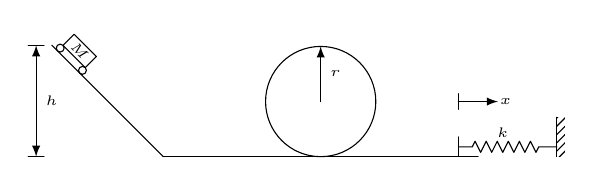
\begin{tikzpicture}[line join = round, line cap = round]
  \begin{scope}[rotate = -45]
    \draw (0, 0) -- (2, 0);
    \draw (.1, .05) circle[radius = .05];
    \draw (.5, .05) circle[radius = .05];
    \draw (.1, .1) rectangle (.5, .3);

    \node[font = \tiny, rotate = -45] at (.3, .2) {$M$};
  \end{scope}
  
  \pgfmathsetmacro{\x}{2*cos(-45)}
  \pgfmathsetmacro{\y}{2*sin(-45)}
  \def\r{.7}

  \draw[latex-latex] (-.2, 0) -- (-.2, \y) node[right, font = \tiny, pos = .5]
  {$h$};
  \draw (-.3, 0) -- (-.1, 0);
  \draw (-.3, \y) -- (-.1, \y);
  \draw (\x, \y) coordinate (P1) -- +(4, 0) coordinate (P2);
  \draw ($(\x, \y) + (2, \r)$) circle[radius = \r];
  \draw[-latex] ($(\x, \y) + (2, \r)$) -- +(0, \r) node[font = \tiny, right,
  pos = .5] {$r$};
  \draw ($(\x, \y) + (3.75, 0)$) -- +(0, .25);
  \draw ($(\x, \y) + (5, 0)$) -- +(0, .5);

  \fill[pattern = north east lines] ($(\x, \y) + (5, 0)$) rectangle
  ($(\x, \y) + (5.1, .5)$);

  \draw[decorate, decoration = {
    zigzag,
    pre length = 5,
    post length = 5,
    segment length = 4,
    amplitude = 2}
  ]
  ($(\x, \y) + (3.75, .125)$) -- ($(\x, \y) + (5, .125)$)
  node[font = \tiny, above, pos = .45] {$k$};
  \draw[-latex] ($(\x, \y) + (3.75, .7)$) -- +(.5, 0) node[font = \tiny,
  pos = 1.2] {$x$};
  \draw ($(\x, \y) + (3.75, .6)$) -- +(0, .2); 
\end{tikzpicture}
\end{document}
%%% Local Variables:
%%% mode: latex
%%% TeX-master: t
%%% End:
